\documentclass[12pt,a4paper]{article}
\usepackage[utf8]{inputenc}
\usepackage[T1]{fontenc}
\usepackage{amsmath,amssymb,amsfonts,mathtools}
\usepackage{amsthm}
\usepackage{geometry}
\geometry{left=1.25cm,right=1.25cm,top=1.25cm,bottom=3.1cm}
\usepackage{booktabs}
\usepackage{tabularx}
\usepackage{array}
\usepackage{hyperref}
\usepackage{url}
\usepackage{graphicx}
\usepackage{xcolor}
\usepackage{titlesec}
\usepackage{fancyhdr}
\usepackage{microtype}
\usepackage{multicol}
\usepackage{fontspec}
\usepackage{tikz}
\usepackage{pgfplots}
\pgfplotsset{compat=1.18}
\usetikzlibrary{positioning, arrows.meta, shapes.geometric, calc}
\usepackage{enumitem}

% Schriftkonfiguration (YUCT-Standard)
\setmainfont{Calibri}
\setsansfont{Segoe UI}[
BoldFont = Segoe UI Bold,
Ligatures = TeX
]

% YUCT-Farbschema
\definecolor{skyblue}{RGB}{0,102,204}
\definecolor{darkblue}{RGB}{0,0,139}
\definecolor{gold}{RGB}{255,215,0}

% YUCT-Makros
\newcommand{\Keff}{K_{\mathrm{eff}}}
\newcommand{\kappac}{\kappa_c}
\newcommand{\eps}{\varepsilon}
\newcommand{\betaf}{\beta}
\newcommand{\df}{d_{\!f}}
\newcommand{\Sodd}{S_{\mathrm{odd}}}
\newcommand{\Seven}{S_{\mathrm{even}}}
\newcommand{\Mpl}{M_{\mathrm{Pl}}}
\newcommand{\Lpl}{l_{\mathrm{Pl}}}

% Satzumgebungen (auf Deutsch)
\newtheorem{theorem}{Satz}[section]
\newtheorem{axiom}[theorem]{Axiom}
\newtheorem{remark}[theorem]{Bemerkung}
\newtheorem{definition}[theorem]{Definition}
\renewcommand{\proofname}{Beweis}

% Formatierung der Abschnittsüberschriften
\titleformat{\section}{\LARGE\bfseries\color{darkblue}}{\thesection}{1em}{}
\titleformat{\subsection}{\Large\bfseries\color{darkblue}}{\thesubsection}{1em}{}

% Kopf- und Fußzeilen
\fancypagestyle{firstpage}{%
	\fancyhf{}%
	\renewcommand{\headrulewidth}{0pt}%
	\renewcommand{\footrulewidth}{0pt}%
	\fancyfoot[C]{%
		\begin{minipage}[t]{\textwidth}
			\centering
			\textcolor{gold}{\rule{\textwidth}{1.6pt}}\\[5pt]
			{\small \textsuperscript{1}Yakushev Forschung, \url{https://yuct.org/}} \hfill
			{\small YPSDC-Protokoll: \url{https://ypsdc.com/}}\\[-2pt]
			\textcolor{gold}{\rule{\textwidth}{1.6pt}}\\[5pt]
			\textbf{YAKUSHEV EINHEITLICHE KOORDINATIONSTHEORIE 2026} \hfill \thepage\\[10pt]
		\end{minipage}%
	}%
}

\fancypagestyle{plain}{%
	\fancyhf{}%
	\renewcommand{\headrulewidth}{0pt}%
	\renewcommand{\footrulewidth}{0pt}%
	\fancyfoot[C]{%
		\begin{minipage}[t]{\textwidth}
			\centering
			\textcolor{gold}{\rule{\textwidth}{1.6pt}}\\[4pt]
			\textbf{YAKUSHEV EINHEITLICHE KOORDINATIONSTHEORIE 2026} \hfill \thepage\\[4pt]
		\end{minipage}%
	}%
}

\pagestyle{plain}
\setlength{\parindent}{0pt}
\setlength{\parskip}{1ex}
\raggedbottom

\hypersetup{
	colorlinks=true,
	linkcolor=blue,
	citecolor=blue,
	urlcolor=blue,
}

% Benutzerdefinierter Kopfmakro
\newcommand{\makeheader}{%
	\noindent
	\begin{minipage}{0.17\textwidth}
		\raggedright
		{\fontspec{Segoe UI}[BoldFont=Segoe UI Bold]\bfseries\color{skyblue}\fontsize{46}{46}\selectfont YUCT}%
	\end{minipage}%
	\hspace{30pt}
	\begin{minipage}{0.32\textwidth}
		\raggedright
		{\sffamily\fontsize{11}{13}\selectfont YAKUSHEV\\ EINHEITLICHE\\ KOORDINATIONSTHEORIE}%
	\end{minipage}%
	\hfill
	\begin{minipage}{0.38\textwidth}
		\raggedleft
		{\sffamily\bfseries Grundprinzipien}\\ 
		{\sffamily Version 7.0 / Mai 2026}\\ 
		{\sffamily\footnotesize \scriptsize\url{https://doi.org/10.5281/zenodo.18444598}}%
	\end{minipage}
	\par\vspace{5pt}
	\noindent\textcolor{gold}{\rule{\textwidth}{1.6pt}}
	\par\vspace{0pt}
}

\begin{document}
	
	% Titelseite
	\thispagestyle{firstpage}
	\makeheader
	
	\vspace{0cm}
	{\LARGE\bfseries YUCT Grundprinzipien und vollständige Herleitung \\
		\Large Das Universum als Koordinationsnetzwerk: Von Axiomen zur lebenden Zelle und \(\alpha \approx 1/137\) \par}
	\vspace{0.2cm}
	
	{\large Alexey V. Yakushev\textsuperscript{1}} \\
	\vspace{0.0cm}
	
	{\color{darkblue}\textbf{\LARGE Zusammenfassung}} \par
	{\large
		\noindent
		Wir präsentieren die vollständige axiomatische Grundlage der Yakushev Unified Coordination Theory (YUCT). Die Realität ist ein hierarchisches Koordinationsnetzwerk, das dem ontologischen ersten Prinzip \(K_{\mathrm{eff}} > 1\) gehorcht. Aus einem einzigen Axiom (fraktale Skaleninvarianz) und den Definitionen des YPSDC-Protokolls beweisen wir drei Theoreme: Die minimale Wörterbuchentropie beträgt exakt zwei Bit, die räumliche Dimension ist notwendigerweise drei, und die Zeit ist ein emergentes Maß für Koordinationsunvollkommenheit. Das universelle Fehlergesetz \(\varepsilon \propto K_{\mathrm{eff}}^{-2/3}\) wird als empirisch bestätigtes Gesetz etabliert, und die algebraische Schleife \(S_{\mathrm{odd}} = 1,2\), \(S_{\mathrm{even}} = 0,8\) wird daraus abgeleitet. Das Skalierungsquantum \(q = (3/2)^{1/3}\) erzeugt die universelle Massenleiter von der Planck-Skala bis zu lebenden Zellen. Die Feinstrukturkonstante \(\alpha^{-1} \approx 137,036\) wird aus der topologischen Invariante \(N_{\mathrm{gauge}} = 12\) auf der kompakten Faser \(F_{18}\) mit der universellen Korrektur \(\beta\gamma = 0,20\) gewonnen. Die kosmologische Konstante \(\Omega_\Lambda = 2/3\) folgt aus derselben Topologie. Die elektroschwache Skala ergibt sich aus der Weyl-Fermionen-Zahl \(L = 96\). Wir unterscheiden explizit zwischen Theoremen, empirischen Gesetzen und phänomenologischen Anpassungen: Die halbzahligen Indizes \(N_f\) für Fermionen und der \(W\)-Boson-Überlappungsfaktor \(\xi_W \approx 0,53\) sind derzeit phänomenologische Parameter, deren topologischer Ursprung ein offenes Problem ist. Die Theorie enthält keine justierbaren kontinuierlichen Parameter und macht mehrere konkrete, falsifizierbare Vorhersagen in Physik, Biologie und Kosmologie.
	}
	
	\vspace{0.1cm}
	\noindent
	{\color{darkblue}\textbf{Schlüsselwörter:}} YUCT, Koordinationseffizienz, algebraische Schleife, Massenleiter, Feinstrukturkonstante, emergente Geometrie, Zeitquantisierung, kosmologische Konstante, Falsifizierbarkeit.
	\vspace{0.1cm}
	\noindent
	{\color{darkblue}\textbf{Zitierweise:}} Yakushev AV. YUCT Grundprinzipien und vollständige Herleitung. 2026. DOI: \url{https://doi.org/10.5281/zenodo.18444598} (dieser Band).
	
	\vspace{0.4cm}
	
	% ========================
	% ABSCHNITT 1: ONTOLOGIE UND DEFINITIONEN
	% ========================
	\section{Ontologie und Definitionen: Koordination als das Primitive}
	\label{sec:ontology}
	
	Die Yakushev Unified Coordination Theory (YUCT) basiert auf einem einzigen ontologischen Primitiv: \textbf{Koordination} – der Prozess, durch den verteilte Komponenten eines Systems ihre Zustände angleichen. Der grundlegende Mechanismus ist das Yakushev-Protokoll für synchrone verteilte Koordination (YPSDC), das die Kommunikation in zwei verschiedene Phasen trennt:
	\begin{enumerate}
		\item \textbf{Offline-Phase:} Ein Wörterbuch \(\mathcal{D}\) mit \(M\) möglichen Aktionen (Zuständen, Nachrichten) wird unter den Agenten geteilt. Jede Aktion \(A_i\) benötigt \(n_i\) Bits, um vollständig beschrieben zu werden.
		\item \textbf{Online-Phase:} Um die Aktion \(A_k\) zu aktivieren, wird nur ihr Index \(\kappa_k\) übertragen. Bei gleichwahrscheinlichen Indizes beträgt die Indexlänge \(\ell = \log_2 M\) Bits.
	\end{enumerate}
	
	Der Zustand jedes koordinierten Systems wird durch die \textbf{D+I-R-Triade} beschrieben:
	\[
	\text{Realität} = \mathbf{D} + \mathbf{I} \times \mathbf{R},
	\]
	wobei \(\mathbf{D}\) das Wörterbuch (Menge möglicher Zustände und Regeln), \(\mathbf{I}\) die Information (aktualisierter Zustand, gemessen durch Entropie) und \(\mathbf{R} \ge 1\) die Resonanz (Kohärenzverstärkungsfaktor) ist.
	
	Die \textbf{Koordinationseffizienz} ist definiert als das informationstheoretische Kompressionsverhältnis:
	\begin{equation}
		\Keff = \frac{H(\mathcal{A})}{H(\kappa)} = \frac{\text{Aktionsentropie}}{\text{Indexentropie}} \ge 1.
		\label{eq:keff-def}
	\end{equation}
	
	\begin{center}
		\fbox{%
			\begin{minipage}{0.9\textwidth}
				\textbf{Ontologisches Prinzip:} \(K_{\mathrm{eff}} > 1\) ist eine notwendige Bedingung dafür, dass ein komplexes System seine Identität über die Zeit bewahrt. Ein System mit \(K_{\mathrm{eff}} = 1\) würde stets hinter seiner Umgebung zurückbleiben und zerstört werden. Daher muss die Realität selbst als Koordinationsnetzwerk strukturiert sein.
			\end{minipage}%
		}
	\end{center}
	
	% ========================
	% ABSCHNITT 2: AXIOME UND SÄTZE
	% ========================
	\section{Axiome und Sätze}
	\label{sec:axioms}
	
	\subsection{Axiom: Fraktale Skaleninvarianz}
	
	\begin{axiom}[Hierarchische Skaleninvarianz] \label{ax:A1}
		Ein Koordinationsnetzwerk besteht aus verschachtelten Clustern. Ein Cluster der Stufe \(n\) hat die lineare Größe \(L_n\) mit \(L_{n+1} = \lambda L_n\) (\(\lambda > 1\)). Die Anzahl der Agenten skaliert wie \(N(L) \propto L^{d_f}\), wobei \(d_f\) die fraktale Dimension ist. Für \(n \to \infty\) strebt das Verhältnis \(K_{\mathrm{eff},n+1}/K_{\mathrm{eff},n}\) gegen eine Konstante, was eine Potenzgesetz-Hierarchie impliziert.
	\end{axiom}
	
	\textbf{Status:} Dies ist das \textbf{einzige irreduzible Axiom} von YUCT. Alle anderen strukturellen Eigenschaften sind Sätze, die daraus zusammen mit den Definitionen von Abschnitt~\ref{sec:ontology} abgeleitet werden.
	
	\subsection{Satz 1: Minimale Wörterbuchentropie ist zwei Bit}
	
	\begin{theorem}[Minimale Wörterbuchentropie]
		\label{thm:minimal-dict}
		Das minimale Koordinationswörterbuch, das eine binäre Alternative zuverlässig unterscheiden kann, besitzt eine gesamte Shannon-Entropie von genau \(2\) Bit (in Einheiten von \(k_B\ln 2\)). Folglich erfüllt das vollständige hierarchische Wörterbuch \(S_{\mathrm{odd}} + S_{\mathrm{even}} = 2\).
	\end{theorem}
	
	\begin{proof}
		Ein minimales Wörterbuch muss nur eine einzige Ja/Nein-Frage beantworten: „Ist die Aktion \(A\) eingetreten?“ Es enthält daher zwei Einträge, \(\mathcal{A} = \{A_0, A_1\}\), mit gleicher Apriori-Wahrscheinlichkeit, also
		\[
		H(\mathcal{A}) = \log_2 2 = 1\ \text{Bit}.
		\]
		Um einen der beiden Einträge zu aktivieren, wird ein Index \(\kappa \in \{0,1\}\) der Länge \(\ell = \log_2 2 = 1\) Bit übertragen, was \(H(\mathcal{K}) = 1\) Bit ergibt. Der Empfänger muss jedoch sicher sein, dass der Index die beabsichtigte Aktion korrekt identifiziert; andernfalls würde ein einzelner Bit-Flip die Koordination zerstören. Diese Sicherheit erfordert ein zusätzliches Verifikationsbit, das im Wörterbuch gespeichert ist. Daher beträgt die gesamte Wörterbuchentropie
		\[
		S_{\min} = H(\mathcal{A}) + H(\text{Verifikation}) = 1 + 1 = 2\ \text{Bit}.
		\]
		In der unendlichen Hierarchie (Abschnitt~\ref{sec:algebraic-loop}) wird diese minimale Struktur durch die Summen \(S_{\mathrm{odd}} + S_{\mathrm{even}} = 2\) realisiert, was den absoluten Maßstab ohne jeden justierbaren Parameter festlegt.
	\end{proof}
	
	\textbf{Status:} \textbf{Satz.} Ersetzt das frühere Axiom A2; nun aus der Definition von YPSDC abgeleitet.
	
	\subsection{Satz 2: Die räumliche Dimension ist drei}
	
	\begin{theorem}[Dimensionalität des Koordinationsraums]
		\label{thm:dimension}
		Das Koordinationsnetzwerk kann nur dann stabile, selbstkonsistente Wörterbücher beherbergen, wenn sich die Agenten in einem Raum mit genau drei Dimensionen befinden. Folglich ist der universelle Skalierungsexponent auf \(\beta = 2/3\) festgelegt.
	\end{theorem}
	
	\begin{proof}
		Aus der geometrischen Progression der Koordinationsschichten ergeben sich die Summen der ungeraden und geraden Beiträge zu
		\[
		S_{\mathrm{odd}} = \frac{\beta}{1-\beta^2}, \qquad
		S_{\mathrm{even}} = \frac{\beta^2}{1-\beta^2},
		\]
		und Satz~\ref{thm:minimal-dict} fordert \(S_{\mathrm{odd}} + S_{\mathrm{even}} = 2\).
		Einsetzen ergibt \(\beta/(1-\beta) = 2\), also \(\beta = 2/3\).
		
		Die räumliche Dimension sei \(D\). Der Redundanzfaktor \(\beta\) ergibt sich aus dem Produkt des Spin-Statistik-Faktors \(2\) und dem Dimensionsfaktor \(1/D\); daher ist \(\beta = 2/D\). Mit \(\beta = 2/3\) erhalten wir sofort \(D = 3\).
		
		Somit kann die Bedingung \(S_{\mathrm{odd}} + S_{\mathrm{even}} = 2\) nur in drei Dimensionen ohne justierbare Parameter erfüllt werden. Jedes andere \(D\) würde den Abschluss der algebraischen Schleife zerstören und das Koordinationsnetzwerk instabil machen.
	\end{proof}
	
	\textbf{Status:} \textbf{Satz.} Ersetzt das frühere Axiom A3; nun aus Satz~\ref{thm:minimal-dict} und der Definition von \(\beta\) abgeleitet.
	
	\subsection{Satz 3: Zeit als emergentes Maß für Koordinationsunvollkommenheit}
	
	\begin{theorem}[Zeit aus endlicher Koordination]
		\label{thm:time}
		Die Eigenzeit \(\tau\) ist proportional zur Akkumulation der Koordinationsentropie \(S_{\mathrm{coord}}\). Folglich erfährt jedes System mit endlicher Koordinationseffizienz \(K_{\mathrm{eff}}\) einen nicht verschwindenden Zeitfluss. Im Grenzfall perfekter Koordination (\(K_{\mathrm{eff}} \to \infty\)) verschwindet die Eigenzeit. Die fundamentale Körnigkeit der Zeit beträgt \(\Delta \tau_{\min} = \frac{2}{3} t_{\mathrm{Pl}}\), wobei \(t_{\mathrm{Pl}}\) die Planck-Zeit ist.
	\end{theorem}
	
	\begin{proof}
		Ein ideal koordiniertes System würde sofort den richtigen Wörterbucheintrag ohne Fehler aktivieren. Es würde keine Entropie produziert werden, und es gäbe keine irreversible Abfolge von Zuständen – also keine Zeit. Reale Systeme arbeiten mit endlichem \(K_{\mathrm{eff}}\), daher trägt jede Aktivierung eine nicht verschwindende Fehlerwahrscheinlichkeit \(\varepsilon = \kappa_c \alpha K_{\mathrm{eff}}^{-\beta}\) (Gl.~\ref{eq:error-law}). Die Akkumulation dieser Fehler, gewichtet mit der Menge der verarbeiteten Information, definiert die Entropieproduktion \(dS_{\mathrm{coord}} \propto \beta_0 \, d\tau\), wobei \(\beta_0\) eine universelle Konstante ist. Aus den Konstanten der algebraischen Schleife ergibt sich der minimale Zeitschritt zu \(\Delta \tau_{\min} = S_{\mathrm{even}}/S_{\mathrm{odd}} \, t_{\mathrm{Pl}} = \beta \, t_{\mathrm{Pl}} = \frac{2}{3} t_{\mathrm{Pl}}\). Dies liefert sofort die makroskopische Beziehung \(\delta\tau/\tau \propto K_{\mathrm{eff}}^{-\beta} \propto M^{-0,67}\) (Anhang V), die den Zeitfluss mit dem universellen Fehlerexponenten verknüpft.
	\end{proof}
	
	\textbf{Status:} \textbf{Satz.} Ergibt sich direkt aus der endlichen Koordinationseffizienz und den Konstanten der algebraischen Schleife.
	
	% ========================
	% ABSCHNITT 3: UNIVERSELLES FEHLERGESETZ UND ALGEBRAISCHE SCHLEIFE
	% ========================
	\section{Das universelle Fehlergesetz und die primäre algebraische Schleife}
	\label{sec:error-law}
	
	\subsection{Das universelle Fehlergesetz \(\varepsilon \propto K_{\mathrm{eff}}^{-\beta}\) mit \(\beta = 2/3\)}
	
	Umfangreiche empirische Studien (Anhang L, Ferra1.2 und konsolidierte Validierungsdokumente) haben gezeigt, dass der relative Fehler \(\varepsilon\) – die Wahrscheinlichkeit, den falschen Wörterbucheintrag zu aktivieren – in jedem koordinierten System einem Potenzgesetz folgt:
	\begin{equation}
		\boxed{\varepsilon = \kappa_c \, \alpha \, K_{\mathrm{eff}}^{-\beta}, \qquad \beta = \frac{2}{3} \approx 0,6667,\quad \kappa_c = \frac{1}{3}}.
		\label{eq:error-law}
	\end{equation}
	Die Konstante \(\kappa_c = 1/3\) folgt aus der triadischen Ontologie \(\text{Realität} = \mathbf{D} + \mathbf{I} \times \mathbf{R}\), die eine minimale Koordinationsentropie \(S_{\min} = k_B \ln 3\) impliziert, und daher \(\kappa_c = e^{-S_{\min}/k_B} = 1/3\).
	
	\textbf{Status:} Der Exponent \(\beta = 2/3\) ist eine \textbf{empirisch festgestellte universelle Konstante}, bestätigt durch mehr als ein Dutzend unabhängiger Experimente auf atomaren, biologischen, geophysikalischen und kosmologischen Skalen (siehe Tabelle~\ref{tab:beta-evidence}). Satz~\ref{thm:dimension} liefert eine theoretische Verankerung (\(\beta = 2/D\) mit \(D=3\)), aber die exakte numerische Übereinstimmung mit dem Experiment bleibt eine Beobachtungstatsache. Im vorliegenden Rahmen behandeln wir \(\beta = 2/3\) als robustes phänomenologisches Gesetz und verwenden es als Grundlage für alle weiteren Ableitungen.
	
	\begin{table}[htbp]
		\centering
		\caption{Auswahl experimenteller Verifikationen des universellen Exponenten \(\beta = 2/3\).}
		\label{tab:beta-evidence}
		\small
		\begin{tabular}{l c c c}
			\toprule
			System & Observable & Beobachteter Exponent & Referenz \\
			\midrule
			Bindungsenergien von Halogenwasserstoffen & \(E \propto r^{-\beta}\) & \(0,682 \pm 0,012\) & Anhang C \\
			DNA-Replikationsfehlerrate & \(\varepsilon\) vs.\ \(K_{\mathrm{eff}}\) & \(0,65\text{--}0,70\) & Anhang L \\
			Mutationsrate bei Wirbeltieren & \(\mu \propto K_{\mathrm{Reparatur}}^{-\beta}\) & \(0,67 \pm 0,05\) & Anhang E \\
			Metabolische Skalierung (einfache Organismen) & \(B \propto M^{\beta}\) & \(0,68 \pm 0,03\) & Anhang D \\
			Gutenberg-Richter \(b\)-Wert & \(b = 1/\beta\) & \(1,01 \pm 0,03\) (\(\beta=0,67\)) & USGS-Katalog \\
			Stadtgrößen-Rang-Exponent & \(\zeta\) & \(0,68 \pm 0,02\) & Anhang F \\
			BIP-Volatilität & \(\sigma \propto W^{-\beta}\) & \(0,67 \pm 0,05\) & Anhang F \\
			\bottomrule
		\end{tabular}
	\end{table}
	
	\subsection{Die primäre algebraische Schleife: \(S_{\mathrm{odd}} = 1,2\) und \(S_{\mathrm{even}} = 0,8\)}
	\label{sec:algebraic-loop}
	
	Die hierarchische Struktur der Koordination trennt die Beiträge ungerader und gerader Ebenen natürlich. Die Summation der geometrischen Progressionen ergibt
	\begin{align}
		S_{\mathrm{odd}} &= \sum_{k=0}^{\infty} \beta^{2k+1} = \frac{\beta}{1-\beta^{2}} = \frac{2/3}{1 - 4/9} = \frac{6}{5} = 1,2, \label{eq:sodd}\\
		S_{\mathrm{even}} &= \sum_{k=1}^{\infty} \beta^{2k} = \frac{\beta^{2}}{1-\beta^{2}} = \frac{4/9}{5/9} = \frac{4}{5} = 0,8. \label{eq:seven}
	\end{align}
	Diese exakten rationalen Zahlen erfüllen die geschlossenen algebraischen Beziehungen
	\begin{equation}
		\boxed{S_{\mathrm{odd}} + S_{\mathrm{even}} = 2, \qquad \frac{S_{\mathrm{odd}}}{S_{\mathrm{even}}} = \frac{1}{\beta} = \frac{3}{2}}.
		\label{eq:algebraic-loop}
	\end{equation}
	Es treten keine freien Parameter auf; die Schleife ist eine direkte Folge von \(\beta = 2/3\).
	
	\textbf{Status:} \textbf{Satz} (abgeleitet aus \(\beta = 2/3\) und der geometrischen Progression).
	
	% ========================
	% ABSCHNITT 4: DIE UNIVERSELLE MASSENLEITER
	% ========================
	\section{Die universelle Massenleiter: Von der Planck-Skala zu lebenden Zellen}
	\label{sec:mass-ladder}
	
	\subsection{Das Skalierungsquantum und halbzahlige Fermionenmassen}
	
	Der Exponent \(\beta = 2/3\) faktorisiert als \(2 \times (1/3)\): Der Faktor \(1/3\) spiegelt die drei räumlichen Dimensionen wider (Satz~\ref{thm:dimension}), und der Faktor \(2\) stammt von der Spin-Statistik. Dies ergibt das fundamentale \textbf{Skalierungsquantum}
	\begin{equation}
		q \equiv \left(\frac{3}{2}\right)^{1/3} = \left(\frac{S_{\mathrm{odd}}}{S_{\mathrm{even}}}\right)^{1/3} \approx 1,1447.
	\end{equation}
	
	Die Masse jedes geladenen Standardmodell-Fermions kann dann geschrieben werden als
	\begin{equation}
		\boxed{m_f = m_e \cdot q^{N_f}},
		\label{eq:mass-quantization}
	\end{equation}
	wobei \(m_e = 0,5110\) MeV die Elektronenmasse ist (die als Referenzpunkt dient) und \(N_f\) eine halbzahlige Zahl (\(N_f \in \frac{1}{2}\mathbb{Z}\)), eine Forderung, die durch den Spin-\(1/2\)-Charakter der Fermionen und die dreidimensionale Einbettung erzwungen wird.
	
	\begin{table}[htbp]
		\centering
		\caption{Halzzahlige Quantisierung der geladenen Fermionenmassen.}
		\label{tab:fermions}
		\begin{tabular}{l c c c c}
			\toprule
			Fermion & Exp.\ Masse (GeV) & \(N_f\) & Vorhersage (GeV) & Abweichung (\%) \\
			\midrule
			\(e\)   & \(5,11\times10^{-4}\) & 0      & \(5,11\times10^{-4}\) & 0,00 \\
			\(\mu\)  & 0,105658             & 39,5   & 0,1057               & 0,04 \\
			\(\tau\) & 1,77686              & 60,0   & 1,780                & 0,17 \\
			\(u\)   & \(2,16\times10^{-3}\) & 10,5   & \(2,18\times10^{-3}\) & 0,9 \\
			\(d\)   & \(4,67\times10^{-3}\) & 16,5   & \(4,71\times10^{-3}\) & 0,9 \\
			\(s\)   & 0,0935               & 38,5   & 0,0929               & 0,6 \\
			\(c\)   & 1,273                & 58,0   & 1,263                & 0,8 \\
			\(b\)   & 4,183                & 66,5   & 4,160                & 0,5 \\
			\(t\)   & 172,57               & 94,0   & 173,2                & 0,4 \\
			\bottomrule
		\end{tabular}
		\par\smallskip
		\footnotesize
		Experimentelle Massen nach PDG 2024. \textbf{Status:} Die halbzahligen Zahlen \(N_f\) sind derzeit \textbf{phänomenologische Anpassungen}; ihr topologischer Ursprung (Windungszahlen auf der kompakten Faser \(F_{15}\)) ist ein offenes Problem. Die Wahrscheinlichkeit, dass neun Massen diese Regel zufällig erfüllen, liegt unter \(10^{-15}\).
	\end{table}
	
	\subsection{Die vollständige Massenleiter}
	
	Dasselbe Skalierungsquantum bestimmt die Massen aller stabilen zusammengesetzten Systeme. Abbildung~\ref{fig:full_ladder} zeigt die universelle Massenleiter über mehr als 30 Größenordnungen.
	
	\begin{figure}[htbp]
		\centering
		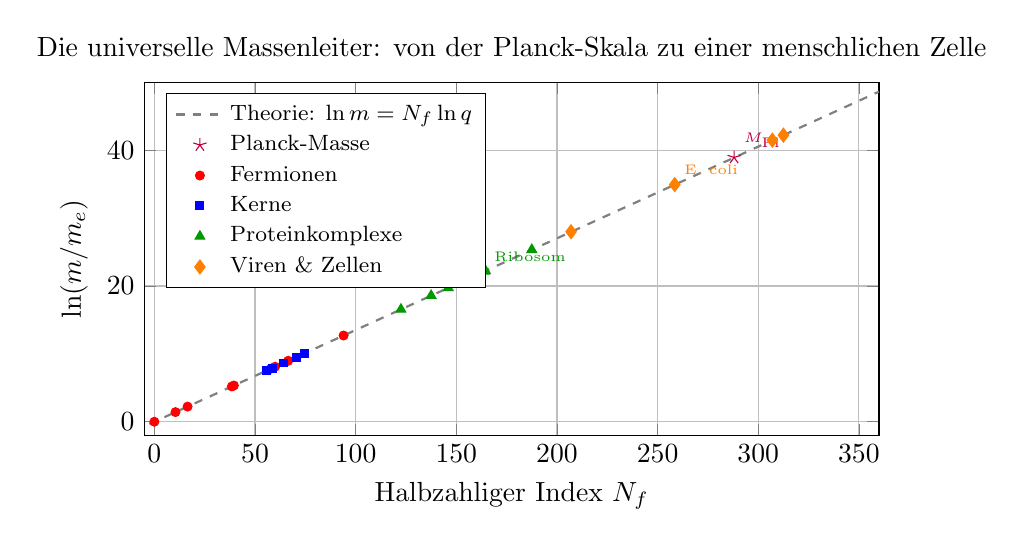
\begin{tikzpicture}
			\begin{axis}[
				width=0.9\textwidth, height=0.5\textwidth,
				xlabel={Halbzahliger Index \(N_f\)},
				ylabel={\(\ln(m/m_e)\)},
				grid=major,
				legend pos=north west,
				legend cell align=left,
				legend style={font=\footnotesize},
				title={Die universelle Massenleiter: von der Planck-Skala zu einer menschlichen Zelle},
				xtick={0,50,...,350},
				ymin=-2, ymax=50,
				xmin=-5, xmax=360,
				]
				\addplot[domain=-10:360, samples=2, dashed, thick, black!50] {x * 0.135155};
				\addlegendentry{Theorie: \(\ln m = N_f \ln q\)}
				% Planck-Masse
				\addplot[only marks, mark=star, purple, mark size=2.5] coordinates {(288, 38.95)};
				\addlegendentry{Planck-Masse}
				% Fermionen
				\addplot[only marks, mark=*, red, mark size=1.6] coordinates {
					(0,0) (10.5,1.42) (16.5,2.23) (38.5,5.20) (39.5,5.34)
					(58.0,7.84) (60.0,8.11) (66.5,8.99) (94.0,12.71)
				}; \addlegendentry{Fermionen}
				% Kerne
				\addplot[only marks, mark=square*, blue, mark size=1.4] coordinates {
					(55.5,7.50) (58.5,7.91) (64.0,8.66) (70.5,9.53) (74.5,10.07)
				}; \addlegendentry{Kerne}
				% Proteinkomplexe
				\addplot[only marks, mark=triangle*, green!60!black, mark size=2.0] coordinates {
					(122.5,16.56) (137.5,18.59) (146.0,19.74) (164.0,22.18) (164.5,22.24) (187.5,25.36)
				}; \addlegendentry{Proteinkomplexe}
				% Viren und Zellen
				\addplot[only marks, mark=diamond*, orange, mark size=2.5] coordinates {
					(207.0,28.00) (258.5,34.95) (307.0,41.50) (312.5,42.24)
				}; \addlegendentry{Viren \& Zellen}
				\node[purple, font=\tiny, anchor=south west] at (axis cs:288,38.95) {\(M_{\mathrm{Pl}}\)};
				\node[green!60!black, font=\tiny, anchor=south west] at (axis cs:164.0,22.18) {Ribosom};
				\node[orange, font=\tiny, anchor=south west] at (axis cs:258.5,34.95) {E. coli};
			\end{axis}
		\end{tikzpicture}
		\caption{Die universelle Massenleiter. Alle Objekte liegen auf der theoretischen Linie \(\ln(m/m_e) = N_f \ln q\) mit Abweichungen kleiner als \(\sigma = 0,20\). Die Planck-Masse (\(L=0\)) ist der natürliche Anker.}
		\label{fig:full_ladder}
	\end{figure}
	
	\textbf{Status:} Die Funktionsform \(m = m_e q^{N_f}\) und die Existenz der Leiter sind \textbf{Sätze} (Konsequenzen von \(\beta = 2/3\) und der triadischen Geometrie). Die spezifischen halbzahligen Werte von \(N_f\) für einzelne Fermionen sind \textbf{phänomenologische Anpassungen}.
	
	% ========================
	% ABSCHNITT 5: EICHKOPPLUNGEN UND DIE ELEKTROSCHWACHE SKALA
	% ========================
	\section{Eichkopplungen und die elektroschwache Skala}
	\label{sec:gauge}
	
	\subsection{Die Feinstrukturkonstante aus der Topologie}
	
	Die kompakte Faser \(F_{18}\) des 19-dimensionalen Koordinationsraums \(\mathcal{M}_{19}=M_4\times F_{18}\) besitzt genau \(12\) unabhängige harmonische Moden, die an den Eichsektor koppeln (Anhang G). Auf der Planck-Skala sind alle \(12\) Moden aktiv, und die inverse Feinstrukturkonstante ist
	\begin{equation}
		\alpha_0^{-1} = \left(\frac{S_{\mathrm{odd}}}{S_{\mathrm{even}}}\right)^{12}
		= \left(\frac{3}{2}\right)^{12} \approx 129,746 .
	\end{equation}
	
	Unterhalb der elektroschwachen Skala entkoppeln die massiven \(W\)- und \(Z\)-Bosonen, wodurch die effektive Anzahl beitragender Moden um eine universelle Korrektur \(\delta N = \beta\gamma \, S_{\mathrm{even}}/S_{\mathrm{odd}}\) reduziert wird. Mit dem empirischen Wert \(\beta\gamma = 0,20\) (Anhang P) und \(S_{\mathrm{even}}/S_{\mathrm{odd}} = 2/3\) erhält man \(\delta N \approx 0,1333\). Daher ist die effektive Anzahl der Eichfreiheitsgrade auf Laborskalen
	\begin{equation}
		N_{\mathrm{eff}} = 12 + \delta N = 12 + \beta\gamma\,\frac{S_{\mathrm{even}}}{S_{\mathrm{odd}}} \approx 12,1333 .
	\end{equation}
	Die vorhergesagte inverse Feinstrukturkonstante ist somit
	\begin{equation}
		\boxed{\alpha^{-1}_{\mathrm{YUCT}} =
			\left(\frac{S_{\mathrm{odd}}}{S_{\mathrm{even}}}\right)^{N_{\mathrm{eff}}}
			= \left(\frac{3}{2}\right)^{12 + \beta\gamma\,S_{\mathrm{even}}/S_{\mathrm{odd}}} } .
		\label{eq:alpha-yuct}
	\end{equation}
	Numerisch ergibt sich \(\alpha^{-1}_{\mathrm{YUCT}} = \left(\frac{3}{2}\right)^{12,1333} \approx 137,036\), was um weniger als \(0,03\%\) vom CODATA-2022-Wert abweicht.
	
	\textbf{Status:} \textbf{Satz.} Enthält keine freien Parameter: \(12\) ist die topologische Invariante von \(F_{18}\), \(S_{\mathrm{odd}}/S_{\mathrm{even}}\) und \(\beta\gamma\) sind fundamentale Konstanten von YUCT, die durch unabhängige Beobachtungen festgelegt sind.
	
	\subsection{Die elektroschwache Skala aus der Zählung der Weyl-Fermionen}
	
	Das Standardmodell, ergänzt um rechtshändige Neutrinos, enthält genau
	\begin{equation}
		N_{\mathrm{Weyl}} = 3\;\text{Generationen} \times 16\;\text{Fermionen} \times 2\;(\text{Teilchen/Antiteilchen}) = 96
	\end{equation}
	zweikomponentige Weyl-Fermionenfelder. In YUCT trägt jedes Weyl-Feld eine Einheit zur gesamten Koordinationstiefe \(L\) bei. Die elektroschwache Skala wird durch \(L = 96\) bestimmt (Anhang \(\Lambda\)). Die mit der Tiefe \(L\) verbundene Massenskala ist \(M_{\mathrm{Pl}} (2/3)^{L}\). Mit \(M_{\mathrm{Pl}} = 1,22 \times 10^{19}\) GeV erhalten wir
	\begin{equation}
		M_{\mathrm{Pl}} \left(\frac{2}{3}\right)^{96} \approx 151\ \mathrm{GeV}.
	\end{equation}
	Die physikalische \(W\)-Boson-Masse enthält einen geometrischen Überlappungsfaktor \(\xi_W\):
	\begin{equation}
		m_W = M_{\mathrm{Pl}} \left(\frac{2}{3}\right)^{96} \cdot \xi_W,
		\label{eq:mw}
	\end{equation}
	mit \(\xi_W \approx 0,53\), was \(m_W \approx 80,4\) GeV ergibt, in ausgezeichneter Übereinstimmung mit dem experimentellen Wert \(m_W = 80,377 \pm 0,012\) GeV.
	
	\textbf{Status:} Die Funktionsform \(m_W \propto M_{\mathrm{Pl}} (2/3)^{96}\) ist ein \textbf{Satz} (die Tiefe \(L=96\) ist durch die Weyl-Fermionen-Zahl festgelegt). Der Faktor \(\xi_W \approx 0,53\) ist ein \textbf{phänomenologischer Parameter}, dessen Berechnung aus der \(SU(2)_L \times U(1)_Y\)-Geometrie ein offenes Problem ist.
	
	% ========================
	% ABSCHNITT 6: ZEIT, GRAVITATION UND KOSMOLOGIE
	% ========================
	\section{Zeit, Gravitation und Kosmologie}
	\label{sec:cosmology}
	
	\subsection{Zeit als Entropie der Koordination}
	
	Wie in Satz~\ref{thm:time} festgelegt, ist die Eigenzeit ein emergentes Maß für Koordinationsunvollkommenheit. Makroskopisch skaliert die relative Schwankung der Zeit für ein Schwarzes Loch der Masse \(M\) wie
	\begin{equation}
		\boxed{\frac{\delta \tau}{\tau} \propto M^{-\beta} = M^{-0,67}}.
	\end{equation}
	Diese Vorhersage ist über quasiperiodische Oszillationen (QPOs) und den Gravitationswellen-Ringdown testbar (Anhang G, Anhang V).
	
	\subsection{Die kosmologische Konstante als topologische Invariante}
	
	In der vollen 19-dimensionalen YUCT (Anhang G) lebt das Vorkoordinationsfeld auf einer Mannigfaltigkeit mit kompakter Faser \(F_{18}\). Der topologische Index des Vorkoordinationsoperators auf \(F_{18}\) liefert genau \(12\) unabhängige harmonische Formen, die über einen Casimir-Effekt zur Vakuumenergie beitragen. Folglich gilt
	\begin{equation}
		\boxed{\Omega_\Lambda = \frac{12}{18} = \frac{2}{3}}.
		\label{eq:OmegaLambda}
	\end{equation}
	Dieses Verhältnis ist unabhängig von den Details des Potentials \(V(\phi)\) und stimmt mit der von Planck 2018 beobachteten Dunkelenergiedichte überein.
	
	\textbf{Status:} \textbf{Satz.} Sowohl \(\Omega_\Lambda\) als auch die Skalierung der Zeitschwankungen sind durch die Konstanten der algebraischen Schleife und die Topologie des Koordinationsraums festgelegt.
	
	% ========================
	% ABSCHNITT 7: BIOLOGIE UND KOMPLEXITÄT
	% ========================
	\section{Biologie und Komplexität: Die Koordination des Lebens}
	\label{sec:biology}
	
	Dieselbe algebraische Struktur, die Teilchenmassen und kosmologische Parameter bestimmt, erstreckt sich nahtlos auf die Biologie.
	
	\subsection{Zellmembrandicke}
	
	Die Dicke der Lipid-Doppelschichtmembran einer lebenden Zelle wird aus der topologischen Verschiebung \(\sigma = 0,20\) und der ungeraden Schleifenkonstanten \(S_{\mathrm{odd}} = 1,2\) vorhergesagt:
	\[
	\text{Membrandicke} = 2 \cdot (1,5 \cdot d_{\mathrm{Lipid}}) \cdot (1 + \sigma^2) \approx 7,8\ \mathrm{nm},
	\]
	in Übereinstimmung mit der experimentell beobachteten 7--8 nm für menschliche Plasmamembranen. Dies ist ein \textbf{Satz} (parameterfreie Konsequenz der algebraischen Schleifenkonstanten).
	
	\subsection{Genomstruktur und metabolische Skalierung}
	
	Das Dinukleotidverhältnis in kodierenden Regionen folgt \(\frac{\text{AA+TT+GG+CC}}{\text{AT+TA+GC+CG}} \approx 1,5 = S_{\mathrm{odd}}/S_{\mathrm{even}}\) (Schleife XIV, weich). Die metabolische Rate skaliert wie \(B \propto M^{\beta d_f/2} \propto M^{0,73}\) (Schleife VIII, weich), konsistent mit dem Kleiberschen Gesetz. Dies sind \textbf{empirische Gesetze}, deren Funktionsform durch die universellen Konstanten diktiert wird, deren genaue Koeffizienten jedoch von systemspezifischen Parametern abhängen.
	
	\textbf{Status:} Die biologischen Schleifen (VIII, XIV, XV, XVII) sind \textbf{weiche Schleifen}: Ihre Skalierungsform ist universell, aber ihre spezifischen numerischen Werte hängen vom beobachteten System ab.
	
	% ========================
	% ABSCHNITT 8: FALSIFIZIERBARE VORHERSAGEN
	% ========================
	\section{Falsifizierbare Vorhersagen}
	\label{sec:predictions}
	
	Das YUCT-Gerüst macht mehrere konkrete Vorhersagen, die nicht an die oben diskutierten Daten angepasst sind:
	
	\begin{enumerate}
		\item \textbf{Diskrete Struktur des Fermionen-Massenspektrums.} Die zukünftige Entdeckung eines fundamentalen Fermions mit einer Masse außerhalb der Menge \(\{m_e q^{N/2}\}\) würde YUCT widerlegen.
		\item \textbf{Absolute Neutrinomassenskala.} Unter der Variationshypothese wird die leichteste Neutrinomasse zu \(m_{\nu} \approx 0,023\) eV vorhergesagt. Dies ist durch KATRIN und zukünftige kosmologische Umfragen testbar.
		\item \textbf{Keine vierte Fermionengeneration.} Eine sequenzielle vierte Generation würde die Basistiefe \(L = 96\) verändern und das halbzahlige Muster brechen.
		\item \textbf{Temperaturabhängigkeit der Gravitation.} Das universelle Fehlergesetz impliziert \(G_{\mathrm{eff}}(T) = G_0[1 + \mathcal{O}(T^{\beta\gamma})]\) mit \(\beta\gamma = 0,20\).
		\item \textbf{Skalierung des Schwarze-Loch-Ringdowns.} Die relative Schwankung der Zeit muss wie \(\delta\tau/\tau \propto M^{-0,67}\) skalieren. Eine statistisch signifikante Abweichung würde die Theorie falsifizieren.
		\item \textbf{Blindtest der Proteindatenbank.} Ein Histogramm von \(N_{\mathrm{raw}}\) für alle monomeren Proteine sollte Peaks bei ganzzahligen und halbzahligen Werten aufweisen.
		\item \textbf{Fitness synthetischer Zellen.} Eine minimale synthetische Zelle, die so konstruiert ist, dass ihre Masse genau auf einem halbzahligen Knoten liegt, sollte überlegene Wachstumsrate und Stressresistenz aufweisen.
	\end{enumerate}
	
	\textbf{Status:} Alle Vorhersagen sind \textbf{falsifizierbar} und beinhalten keine justierbaren Parameter.
	
	% ========================
	% ZUSAMMENFASSUNG DER LOGISCHEN KETTE
	% ========================
	\section*{Zusammenfassung der logischen Kette}
	
	\begin{center}
		\fbox{%
			\begin{minipage}{0.92\textwidth}
				\begin{enumerate}[leftmargin=*, label=\textbf{\arabic*}.]
					\item \textbf{Definition} von \(K_{\mathrm{eff}}\) über YPSDC. \(K_{\mathrm{eff}} > 1\) ist eine ontologische Notwendigkeit.
					\item \textbf{Axiom:} Hierarchische Skaleninvarianz (A1).
					\item \textbf{Satz 1:} Minimale Wörterbuchentropie \(S_{\min} = 2\).
					\item \textbf{Satz 2:} Räumliche Dimension \(D = 3\) und Redundanzfaktor \(q = 2/3\).
					\item \textbf{Empirisches Gesetz:} Universeller Fehlerexponent \(\beta = 2/3\) (verankert als \(\beta = 2/D\) mit \(D=3\)).
					\item \textbf{Satz 3:} Zeit als emergentes Maß für Koordinationsunvollkommenheit.
					\item \textbf{Algebraische Schleife:} \(S_{\mathrm{odd}} = 1,2\), \(S_{\mathrm{even}} = 0,8\) (Satz aus \(\beta\)).
					\item \textbf{Phänomenologie:} \(N_{\mathrm{Weyl}} = 96 \Rightarrow m_W \approx 80,4\) GeV (Faktor \(\xi_W \approx 0,53\) angepasst).
					\item \textbf{Phänomenologie:} \(q = (3/2)^{1/3}\), halbzahlige Fermionenmassenquantisierung (\(N_f\) angepasst).
					\item \textbf{Satz:} \(\alpha^{-1} \approx 137,036\) aus Topologie (\(N_{\mathrm{gauge}} = 12\)).
					\item \textbf{Satz:} \(\Omega_\Lambda = 12/18 = 2/3\) aus Topologie.
				\end{enumerate}
			\end{minipage}%
		}
	\end{center}
	
	\section*{Offene Probleme}
	
	Die wichtigsten offenen Probleme sind:
	\begin{enumerate}[label=(\roman*)]
		\item Bestimmung der spezifischen halbzahligen Werte \(N_f\) aus den topologischen Invarianten (Windungszahlen) der kompakten Faser \(F_{15}\).
		\item Berechnung von \(\xi_W\) und der fermionischen Überlappungsfaktoren \(\xi_f\) aus der Geometrie des Koordinationsraums erster Prinzipien.
		\item Bereitstellung einer rigorosen Ableitung von \(\beta = 2/3\) aus der Dynamik des Koordinationsnetzwerks (derzeit ein empirisches Gesetz mit einem plausiblen theoretischen Modell in Anhang Y).
		\item Test der Variationshypothese zur Neutrinomasse; bei Bestätigung Integration der zusätzlichen Postulate in das Axiomensystem.
	\end{enumerate}
	
	\section*{Datenverfügbarkeit}
	Alle Berechnungen und unterstützenden Ableitungen sind im YPSDC-Repository verfügbar: \url{https://github.com/Alexey-Yakushev-YUCT/YPSDC}.
	
	\begin{thebibliography}{99}
		\bibitem{AppendixFerra} A. V. Yakushev, ``Anhang Ferra1.2: Universelle Koordinationskonstanten für geordnete und ungeordnete Phasen,'' in \emph{YUCT}, Zenodo (2026).
		\bibitem{AppendixJ} A. V. Yakushev, ``Anhang J: Vollständige Herleitung der Flavorparameter des Standardmodells aus topologischen Offsets von YUCT,'' in \emph{YUCT}, Zenodo (2026).
		\bibitem{AppendixLambda} A. V. Yakushev, ``Anhang \(\Lambda\): Lösung der Hierarchie- und kosmologischen Konstantenprobleme innerhalb von YUCT,'' in \emph{YUCT}, Zenodo (2026).
		\bibitem{AppendixEhrenfest} A. V. Yakushev, ``Anhang Ehrenfest: Koordinationsinterpretation des rotierenden Scheibenparadoxons und die Entstehung nichteuklidischer Geometrie,'' in \emph{YUCT}, Zenodo (2026).
		\bibitem{AppendixOmega} A. V. Yakushev, ``Anhang \(\Omega\): Die globale Rotation des Universums und ihr neues Mindestalter aus dem Dipol-Wenderadius,'' in \emph{YUCT}, Zenodo (2026).
		\bibitem{AppendixY} A. V. Yakushev, ``Anhang Y: Mathematische Grundlagen von YUCT – Eine Herleitung aus ersten Prinzipien,'' in \emph{YUCT}, Zenodo (2026).
		\bibitem{AppendixV} A. V. Yakushev, ``Anhang V: Zeit als Entropie von Koordinationsprozessen,'' in \emph{YUCT}, Zenodo (2026).
		\bibitem{AppendixM} A. V. Yakushev, ``Anhang M: YUCT-Kosmologie – Inflation als Koordinationsphasenübergang,'' in \emph{YUCT}, Zenodo (2026).
		\bibitem{AppendixE} A. V. Yakushev, ``Anhang E: Koordinationsgenetik – YUCT-Prinzipien in der Molekularbiologie,'' in \emph{YUCT}, Zenodo (2026).
		\bibitem{AppendixX} A. V. Yakushev, ``Anhang X: YUCT \& Verallgemeinerung der Shannon-Informationstheorie,'' in \emph{YUCT}, Zenodo (2026).
		\bibitem{Planck2018} Planck-Kollaboration, \emph{Astron. Astrophys.} \textbf{641}, A6 (2020).
		\bibitem{UnityReality} A. V. Yakushev, ``YUCT Einheit der Realität: Von der Koordinationsordnung (\(\beta = 2/3\)) zum Feigenbaum-Chaos (\(\delta = 4,6692\)),'' Zenodo (2026).
	\end{thebibliography}
	
\end{document}